
\documentclass[12pt,a4paper]{article}

%======Usepackage=========
\usepackage[utf8]{inputenc}
\usepackage[ngerman]{babel}
\usepackage{graphicx}
\usepackage{hyperref}
\usepackage[square,sort,comma,numbers]{natbib}
\usepackage{tabularx}
\usepackage{fancyhdr}
\usepackage[T1]{fontenc}
\usepackage{lscape}
\usepackage[onehalfspacing]{setspace}
\usepackage{amssymb}
\usepackage{amsmath}
\usepackage[locale=DE]{siunitx}
\usepackage[printonlyused]{acronym}
\usepackage[table]{xcolor}
\usepackage{eurosym}
\usepackage{listings}
\usepackage{pdfpages}

\lstdefinestyle{customc}{
numbers  = left,
numberstyle=\tiny,
numbersep=5pt,
numberblanklines=true,
basicstyle=\sffamily\small,
frame=lines,
showstringspaces = false,
  %belowcaptionskip=1\baselineskip,
  breaklines=true,
  %frame=L,
  xleftmargin=\parindent,
  %language=java,
  %showstringspaces=false,
  %basicstyle=\footnotesize\ttfamily,
  keywordstyle=\bfseries\color{green!40!black},
  commentstyle=\itshape\color{purple!40!black},
  identifierstyle=\color{blue},
  stringstyle=\color{orange},
  abovecaptionskip=\baselineskip,
  captionpos=b
}

%=====Allgemeine Angaben======
\title{Bachelorarbeit}
\author{Marvin Böck}
\date{\today}
\newcommand{\Autor}{Marvin Böck}
\newcommand{\MatrikelNummer}{1892597}
\newcommand{\Kursbezeichnung}{Tinf18B3}


\newcommand{\FirmenName}{SICK STEGMANN GmbH}
\newcommand{\FirmenLogoDeckblatt}{
\includegraphics[width=3cm]{img/Sick_logo.png}}
\newcommand{\FirmenStadt}{Donaueschingen}
\newcommand{\BetreuerFirma}{Timo Bayer, M.Sc.}
\newcommand{\BetreuerDHBW}{Prof. Dr. Hans-Jörg Haubner}
\newcommand{\Titel}{Konzeption und Implementierung einer modularen Testsuite
zur Automatisierung von Softwaretests}
\newcommand{\Untertitel}{Test}
\newcommand{\ModulName}{B-FMP02XX}
\newcommand{\AbgabeDatum}{07. Juli 2022}

\newcommand{\Dauer}{6. Praxisphase}
\newcommand{\Abschluss}{Bachelor of Science}

\newcommand{\Studiengang}{Informatik / Informationstechnik}
\newcommand{\Anschrift}{Solweg 5, 78647 Trossingen}

%======Kopf/Fußzeile=====
\pagestyle{fancy}

    \lhead{}
    \chead{}
    \rhead{\slshape \leftmark}

    \lfoot{}
    \cfoot{\thepage}
    \rfoot{}
    
    \renewcommand{\headrulewidth}{0.4pt}
    \renewcommand{\footrulewidth}{0.4pt}


\bibliographystyle{IEEEtran}    
%======Dokument=======
\begin{document}

%=====deckblatt, Abstrackz/Verzeichnisse======
\pagestyle{empty}
%%\maketitle
\singlespacing
\begin{center}
%\hspace{-2mm} 
\includegraphics[scale=0.15]{img/wbh_logo.jpg}
\FirmenLogoDeckblatt\hfill
\includegraphics[width=4cm]{img/wbh_logo.jpg}\\[2cm]
{\Huge \Titel}\\[1cm]
%{\Huge\scshape \Was}\\[1cm]
{\large für die Prüfung zum}\\[0.5cm]
{\Large \Abschluss}\\[0.5cm]
{\large des Studienganges \Studiengang}\\[0.5cm]
{\large an der}\\[0.5cm]
{\large Dualen Hochschule Baden-Württemberg Karlsruhe}\\[0.5cm]
{\large von}\\[0.5cm]
{\large\bfseries \Autor}\\[1cm]
{\large Abgabedatum \AbgabeDatum}
\vfill

\begin{tabular}{l@{\hspace{2cm}}l}
Bearbeitungszeitraum	         & \Dauer 			\\
Matrikelnummer	                 & \MatrikelNummer		\\
Kurs			         & \Kursbezeichnung		\\
Ausbildungsfirma	         & \FirmenName			\\
			         & \FirmenStadt			\\
Betreuer der Ausbildungsfirma	 & \BetreuerFirma		\\
Gutachter der Studienakademie	 & \BetreuerDHBW		\\
\end{tabular}
\end{center}
 %Für große Arbeiten wie z.B. Masterthesis
%\maketitle
\singlespacing
\begin{center}
%\FirmenLogoDeckblatt\hfill
\includegraphics[width=4cm]{img/wbh_logo.jpg}\\[2cm]
\hfill
\includegraphics[width=4cm]{img/wbh_logo.jpg}\\[2cm]
{\Huge \Titel}\\[1cm]
%{\Huge\scshape \Was}\\[1cm]
{\Large \Untertitel}\\[0.5cm]
{\Large Fachbereich Informatik}\\[0.5cm]
{\large \ModulName}\\[0.5cm]

\vfill

\begin{tabular}{l@{\hspace{2cm}}l}
Autor	 & \Autor		\\
Matrikelnummer	                 & \MatrikelNummer		\\
Anschrift 	& \Anschrift \\
Abgabedatum	 & \AbgabeDatum		\\

\end{tabular}
\end{center}
 %Für kleine Arbeiten, Berichte etc.
\pagenumbering{Roman}
\onehalfspacing
\section*{Erklärung an Eidesstatt}

Hiermit erkläre ich, dass ich die vorliegende Abschlussarbeit mit dem Titel:
\newline
	''\textit{\Titel{}}''
\newline
eigenständig und ohne fremde Hilfe angefertigt habe. Textpassagen, die wörtlich oder dem Sinn nach auf Publikationen oder Vorträgen anderer Autoren beruhen, sind als solche kenntlich gemacht. Die Arbeit wurde bisher keiner anderen Prüfungsbehörde vorgelegt und auch noch nicht veröffentlicht.
\newline
Ich versichere zudem, dass die eingereichte elektronische Fassung mit der gedruckten
Fassung übereinstimmt.

\vspace{4cm}
\parbox{5cm}{\centering \dotfill\\
\centering \footnotesize Ort, Datum} \hfill\parbox{5cm}{\dotfill\\
\centering \footnotesize Unterschrift}



\section*{Sperrvermerk}
Der Inhalt der Arbeit darf weder als Ganzes noch in Auszügen Personen außerhalb des Prüfungsprozesses und des Evaluationsverfahrens zugänglich gemacht werden, sofern keine anderslautende Genehmigung der SICK STEGMANN GmbH vorliegt
\newline


\onehalfspacing
\section*{Zusammenfassung}
Die vorliegende Arbeit befasst sich mit der Kozeptionierung sowie Proof of Concept Implementierung einer modularen Testsuite für Softwaretests. Grund für die Entwicklung der Suite ist die Portierung eines Bestandsprodukts auf eine neue Mikrocontroller Generation und der damit verbundener erhöhter Testaufwand. Bei der Firma SICK STEGAMNN GmbH ist seit kurzem ein Framework zum automatischen Testen von Software im Einsatz welches die Möglichkeit bietet, entsprechende Softwaretests komfortabel abzudecken. Um die Generierung der Testfälle für das Portierungsprojekt zu erleichtern, soll im Rahmen dieser Arbeit eine Testsuite konzeptioniert, sowie prototypisch implementiert werden. Ziel hierbei ist es, den späteren Prozess der Testentwicklung zu beschleunigen, sowie die Testfiles übersichtlicher und robuster zu gestalten. Zu Beginn der Arbeit wird sich ein Überblick über den Bereich Automated Testing @ GBC07 sowie Software Tests im Embedded Bereich geschaffen. Im Anschluss daran, werden die Testfälle eines vergleichbaren Produkts analysiert und geeignete Testfälle identifiziert. Danach wird eine Softwarearchitektur für die Suite konzeptioniert und diese prototypisch implementiert. Zum Schluss werden die Ergebnisse der Arbeit evaluiert.
\newpage
\section*{Abstract}
This thesis deals with the conceptual design and proof of concept implementation of a modular test suite for software testing. The reason for the development of the suite is the porting of an existing product to a new microcontroller generation and the associated increased test effort. The company SICK STEGAMNN GmbH has recently implemented a framework for automatic software testing which offers the possibility to comfortably cover the corresponding software tests. In order to facilitate the generation of test cases for the porting project, a test suite is to be conceptualized and prototypically implemented within the scope of this work. The goal is to accelerate the later process of test development and to make the test files clearer and more robust. At the beginning of the work, an overview of the area of Automated Testing @ GBC07 and software tests in the embedded area is created. Subsequently, the test cases of a comparable product are analyzed and suitable test cases are identified. Afterwards a software architecture for the suite is conceptualized and prototypically implemented. Finally, the results of the work are evaluated.


\singlespacing
%=====Inhaltsverzeichniss===
\tableofcontents
\newpage
%====Abbildungsverzeichniss===
\listoffigures
\newpage
%====Tabellenverzeichniss===
\listoftables
\newpage
%====Listings====
\lstlistoflistings
\newpage
%===Abkürzungsverzeichnis===
\newpage
\section*{Abkürzungsverzeichnis}
	\begin{acronym}[slmtA]
		\acro{MFB}{Motor-Feedback-System}
		\acro{SRS}{Software Requirements Specification}
		\acro{RUP}{Rational Unified Process}
		\acro{CCE}{Continuous and Customised Engineering}
		\acro{LOC}{Lines of Code}
	\end{acronym}

%====Text=============
\newpage
\pagenumbering{arabic}
\pagestyle{fancy}
\newpage
\onehalfspacing

\section{Einleitung}

		\subsection{SICK}

\onehalfspacing
\section{Related Work}
In diesem Kapitel werden verschiedene Literaturquellen diskutiert, welche im Zusammenhang mit dem Thema der Arbeit stehen. Hierbei wird der Inhalt kurz zusammengefasst und erläutert, in welchem Zusammenhang die Arbeiten stehen.
\subsection*{Optimized test suites for automated testing using different optimization techniques}
In diesem Artikel, welcher von Manju Khari, Prabhat Kumar, Daniel Burgos und Rubén González Crespo geschrieben wurde, befassen sich die Autoren mit der Optimierung von automatisierten Testsuites unter Betrachtung verschiedener Optimierungstechniken. Hierbei werden Tools zur automatischen Generierung von Testsuites verglichen. Die Ergebnisse werden dann im Kontext des Automated Testing betrachtet. Die Arbeit zeigt auf, welche Möglichkeiten bei der Optimierung und automatischen Generierung von Softwaretests bestehen. Im Zuge des konkreten Projekts wird ebenfalls eine Testsuite erstellt. Die Betrachtung von eventuellen Optimierungsmöglichkeiten ist für den späteren Verlauf des Projekts durchaus von Interesse.\cite{ManjuKhariPrabhatKumarDanielBurgosRubenGonzalezCrespo.2017}

\subsection*{Eine Technologe für das durchgängige und automatisierte testen eingebetteter Software}
Die Arbeit, welche durch Dipl.-Inform. Till Fischer im Rahmen seiner Dissertation an der Fakultät für Elektrotechnik und Informationstechnik des Karlsruher Instituts für Technologie (KIT)durchgeführt wurde, werden neben den Grundlagen des Testens von eingebetteten Systemen auch die verschiedenen Testebenen diskutiert. Ziel der Arbeit ist die Verbesserung der Durchgängigkeit des Testprozesses für eingebettete Systeme. Als Lösungsstrategie wird durch Fischer eine Testlösung versiert, welche den Quelltext der ausgeführten Software, die Netzwerkkommunikation, sowie das physikalische Verhalten an elektrischen Schnittstellen und der simulierten Umgebung abdeckt. Hier ist der Bezug zum in dieser Arbeit behandelten Automated Testing @ GBC07 Projekt zu erkennen. \cite{Dipl.Inform.TillFischer.2016}



\onehalfspacing
\section{Grundlagen Softwareentwicklung und Verifikation}

\onehalfspacing
\section{Anforderungen}
	\subsection{Anforderungsdefinition}
Zu Beginn des Projekts werden die konkreten Anforderungen an die Suite mit dem Auftraggeber abgestimmt und in Form einer Tabelle Festgehalten. Dieses Vorgehen erleichtert die Endabnahme des Projekts, da die Anforderungen klar definiert und beiden Parteien bekannt sind. Auf die Erstellung eines gesamten \ac{SRS} wird im Rahmen dieses Projekt aus Zeitgründen bewusst verzichtet. Bei den Anforderungen wird zwischen funktionalen und nicht-funktionalen unterschieden. Funktionale Anforderungen sind all jene, welche eine konkrete Funktion der Software definieren. Nicht Funktionale Anforderungen sind Anforderungen wie z.B. Zuverlässigkeit und Zeitverhalten. Die Anforderungen sind in den Tabellen \dq \nameref{tab:Anforderungstabelle}\dq und \dq \nameref{tab:Anforderungstabelle2}\dq dargestellt.
\newpage
\begin{table}[h]
\begin{center}
\begin{tabularx}{\textwidth}{|c|X|X|c|}
\hline
Nr. & Bezeichnung & Beschreibung & Zuordnung \\
\hline
F01 & Error Codes & Eignung zur Stimulation der verschiedenen Fehlerfälle und  dadurch Produktion der entsprechenden Fehlermeldungen (01h-23h) & Funktional \\
\hline
F02 & Identifikation des DUT & Überprüfung der Firmware Version, des elektronischen Typenschilds auf Korrektheit & Funktional \\
\hline
F03 & Diagnose Funktionalität & Überprüfung der vorhandenen Diagnose Funktionalität (z.B. Spannungs Monitoring) & Funktional \\
\hline
F04 & Core Funktionalität & Prüfung der externen Temperatur Schnittstelle, sowie der Single und multiturn Positionsbestimmung & Funktional \\
\hline
F05 & Schnittstellen Config & Auslesen und überprüfen der Schnittstellen Parametrisierung und Funktionalität & Funktional \\
\hline
F06 & Hiperface Befehle & Überprüfung der Funktion der verschiedenen Hiperface Befehle sowie der entsprechnden Antwort & Funktional \\
\hline
F07 & Integration in Automated Testing & Die Suite muss in das Projekt "Automated Testing" Integrierbar sein (Implementierung in ITE, Aufbau nach Vorgaben des Projekts) & Funktional \\
\hline
\end{tabularx}
\end{center}
\caption{Anforderungen funktional \label{tab:Anforderungstabelle}}
\end{table}

\begin{table}[h]

\begin{center}

\begin{tabularx}{\textwidth}{|c|X|X|c|}

\hline
Nr. & Bezeichnung & Beschreibung & Zuordnung \\
\hline
NF01 & Externes Equipment & Möglichkeit zur Integration des am Teststand vorhandenen externe Equipment & Nicht Funktional \\
\hline
NF02 & Universell einsetzbar & Der Aufbau der Suite soll so gestaltet sein, das diese auch zukünftig für die Portierung anderer (ähnlicher) Produkte genutzt werden kann & Nicht Funktional \\
\hline
NF03 & Coding Guidelines & Der Aufbau der Suite soll so gestaltet sein, das diese auch zukünftig für die Portierung anderer (ähnlicher) Produkte genutzt werden kann & Nicht Funktional \\
\hline


\end{tabularx}
\caption{Anforderungen nicht-funktional \label{tab:Anforderungstabelle2}}
\end{center}
\end{table}
\cleardoublepage

\subsection{Analyse bisheriger Testfälle}
Zu Ermittlung der Testfälle welche durch die Suite abgedeckt werden sollen werden die bisherigen Testpläne analysiert. Schwierigkeit hierbei ist, dass der Geber vor ca. 20 Jahren entwickelt wurde. Zum Entwicklungszeitpunkt fand keine, den heutigen Standards entsprechende Dokumentation der Testfälle (Testplan) statt, weiterhin ist zum Projektstart noch kein Testplan für Portierung des Controllers vorhanden. Aus diesem Grund wird für die Analyse der Testfälle auf den Testplan eines ähnlichen Produktes (SEY) welches ebenfalls über eine Hiperface Schnittstelle verfügt zurück gegriffen.\newline
	Die im Testplan festgelegten Tests werden in eine Excel Tabelle übertragen, die Testfälle sind im Testplan in verschiedene Kategorien unterteilt (z.B. General Requirements, HW Architecture, functional Requirements). Da der SEY über zwei Mikrocontroller verfügt (Master und Slave) der SK jedoch nicht werden daraufhin die Testfälle des Slave Microcontrollers aus dem Testplan gestrichen. In einem Zweite Schritt wird die Beschreibung jedes Testfalls Analysiert und geprüft ob dieser Testfall automatisierbar ist. Ein Beispiel für einen nicht automatisierbaren Testfall ist z.B. beim Eingriff mittels Debugger während des Tests gegeben. Die verbleibenden Tests werden mit dem Zuständigen SW-Entwickler besprochen und ggf. angepasst um im folgenden als Grundlage für die Kozeptionierung dienen zu können. Die Entwicklung eines kompletten Testplans für die Portierung wird hierbei nicht forciert, da hierzu der Zeitliche Rahmen nicht gegeben ist. Die 
Analyse der Testfälle zeigt, das sich die Suite besonders für das Testen der Hiperface Schnittstelle eignet. Hier können die verschiedenen Befehle der Schnittstelle gut abgebildet werden. Die Ergebnisse der Analyse sind in \dq \nameref{fig:Analyse.jpg}\dq   Beispielhaft dargestellt und befinden sich im Anhang. Die Farbgebung der Tabelle entspricht den Testfall Clustern.
\begin{figure}[h]
	\centering
  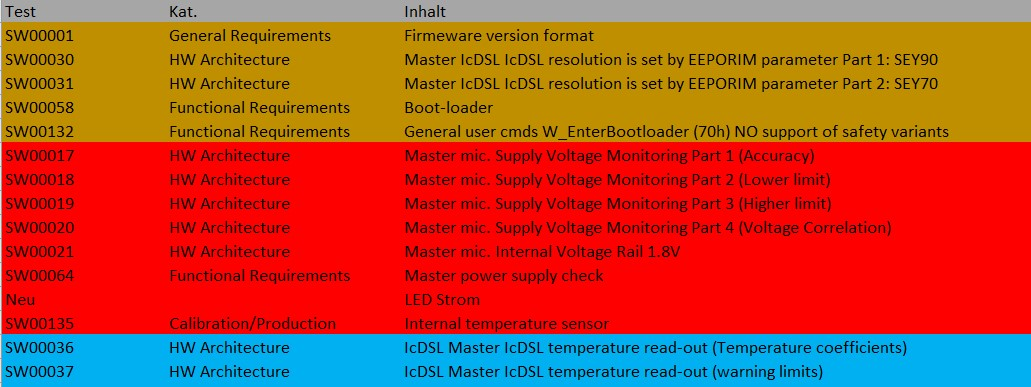
\includegraphics[width=1.25\textwidth, angle=90]{img/Tests_Cluster.jpg} 
   \caption{Tabelle mit Analysierten Testfällen}
  \label{fig:Analyse.jpg}
\end{figure}


\onehalfspacing
\section{Konzept}

\onehalfspacing
\section{Implementierung}

\onehalfspacing
\section{Evaluation}

\onehalfspacing
\section{Fazit / Ausblick}


\pagenumbering{Roman}
\onehalfspacing
\section{Literatur}
	\bibliography{Literatur}
\onehalfspacing
\section{Anhang}







%=====Anhang====



\end{document}
